\section{Convolutional Networks}
\begin{multicols}{2}
	\subsection{The Convolution Operation}
	Convolutional Neural Networks (CNNs) are a kind of neural networks for processing data that has a known, grid-like topology.
	Examples include time-series data, which can be thought of as a 1D grid taking samples at regular time intervals, and image data, which can be thought of as a 2D grid of pixels.
	They are very popular for image processing and hence the both often refer to images and pixels, but they can be used for any dimensional input.\\

	The name CNN indicates that the network employs a mathematical operation called \textbf{convolution}.
	Convolutional networks are neural networks that use convolution in place of general matrix multiplication in at least one of their layers.\\

	If we have a 1D measurement over time and we want to reduce the noise, we can average the sampled data.
	More recent measurements are more relevant, so we will want this to be a weighted average that gives more weight to recent measurements.
	We can do this with a weighting function $w(a)$, where $a$ is the age of a measurement point:
	\[ s(t) = \int x(a)w(t-a)da \]
	If we apply such a weighted average operation at every moment, we obtain a new function $s$ providing a smoothed estimate of the position:
	\[ s(t) = (x\ast w)(t) \]

	$w()$ needs to be a valid probability density function, otherwise the output is not a weighted average.
	$w()$ also needs to be zero for all negative arguments, otherwise it will look into the future (acausal).\\
	If we work with sampled data, we need to work with discrete convolution, hence $t$ and $a$ are now integers and the integral becomes a summation
	\[ s(t) = (x\ast w)(t) = \sum_{a=-\infty}^{\infty} x(a)w(t-a) \]

	We often use convolutions over more than one axis at a time.
	For example, if we use a two-dimensional image $\mI$ as our input, we probably also want to use a two-dimensional kernel $\mK$.
	\begin{align*}
		S(i,j)
		&= (I\ast K)(i,j) &= \sum_m\sum_n I(m,n) K(i-m,j-n)\\
		&= (K\ast I)(i,j) &= \sum_m\sum_n I(i-m,j-n) K(m,n)
	\end{align*}

	Usually the formula in the last line is more straightforward to implement, because there is less variation in range of valid values of $m$ and $n$.
	\begin{figure}[H]
		\centering
		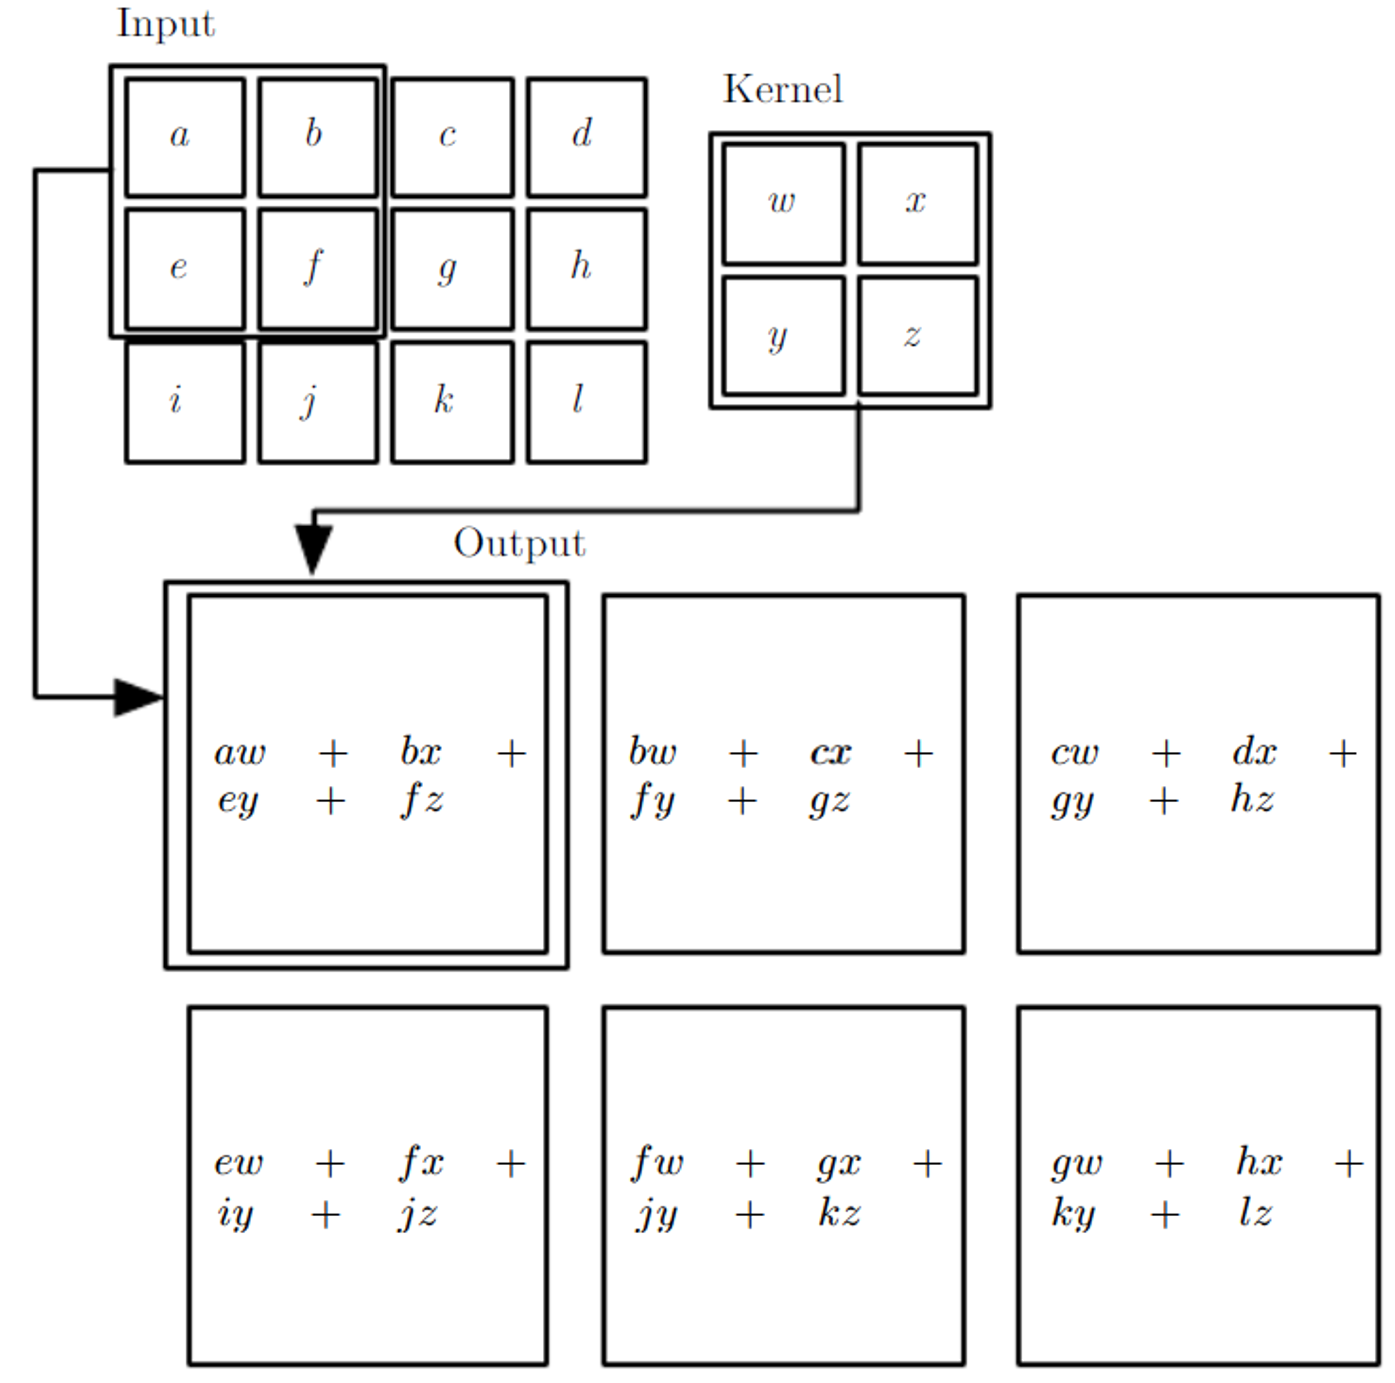
\includegraphics[width=0.65\linewidth]{images/2dconv.PNG}
	\end{figure}
	\subsection{Motivation}
	CNNs typically have \textbf{sparse interactions} (also referred to as sparse connectivity or sparse weights).
	This is accomplished by making the kernel smaller than the input.
	\begin{figure}[H]
		\centering
		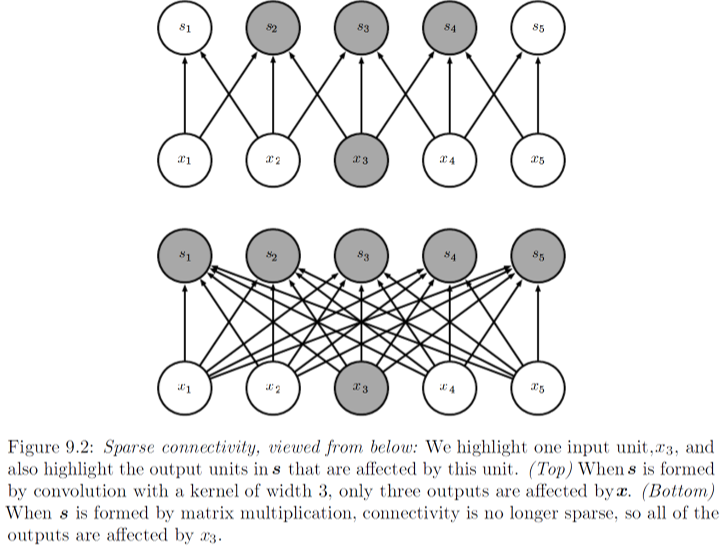
\includegraphics[width=0.85\linewidth]{images/sparse1.png}
	\end{figure}
	\begin{figure}[H]
		\centering
		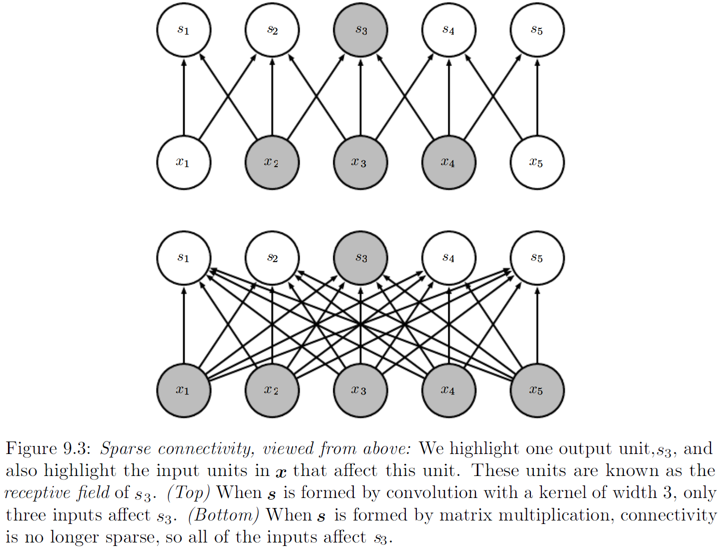
\includegraphics[width=0.85\linewidth]{images/sparse2.png}
	\end{figure}

	\textbf{Parameter Sharing} refers to using the same parameter for more than one function in a model.
	In a traditional neural net, each element of the weight matrix is used exactly once when computing the output of a layer.
	In a CNN, each member of the kernel is used at every position of the input.
	The parameter sharing used by the convolution operation means that rather than learning a separate set of parameters for every location we learn only one set.\\

	This does not affect the runtime of forward propagation but it does further reduce the storage requirements of the model to $k$ parameters.
	Convolution is thus dramatically more efficient than dense matrix multiplication in terms of the memory requirements and statistical efficiency.\\

	Convolution is \textbf{equivariant to translation}.
	This implies that when the input is moved by a certain amount, the output of the convolution is also moved by the same amount in the same direction.
	When processing time series data, this means that convolution produces a sort of timeline that shows when different features appear in the input.
	If we move an event later in time in the input, the exact same representation of it will appear in the input, just later in time.\\
	Similarly with images, convolution creates a 2D map of where certain features appear in the input. If we move the object in the input, its representation will move the same amount in the output.\\

	\subsection{Pooling}
	A typical layer of a CNN consists of three stages:
	\begin{itemize}
		\item In the first stage, the layer performs several convolutions in parallel to produce a set of linear activations
		\item In the second stage, each linear activation is run through a nonlinear activation function, such as the rectified linear activation function (detector stage)
		\item In the third stage, we use a pooling function to modify the output of the layer further. A pooling function replaces the output of the net at a certain location with a \textbf{summary statistic} of the nearby outputs
	\end{itemize}
	Typical pooling function over (mostly rectangular) neighborhoods:
	\begin{itemize}
		\item \textbf{Max pooling} Reports the maximum output
		\item\textbf{Average pooling} Reports the average output
		\item\textbf{Weighted average pooling} Reports a weighted average based on the distance from the central point
		\item\textbf{$L^2$ norm pooling} Reports the $L^2$ norm of a neighborhood
	\end{itemize}
	Pooling helps to make the representation become approximately invariant to small translations of the input.
	If we pool over the outputs of separately parametrized convolutions, the features can learn which transformations to become invariant to.
	\begin{figure}[H]
		\centering
		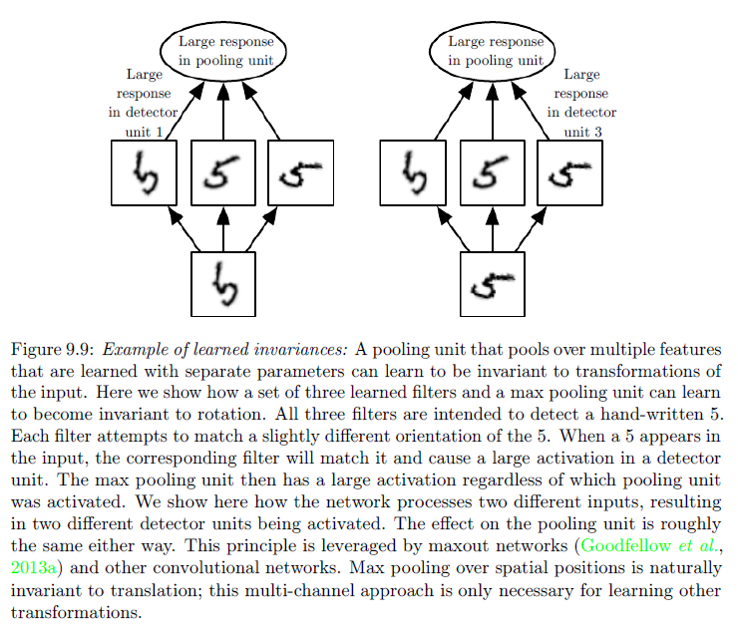
\includegraphics[width=0.8\linewidth]{images/pooling.png}
	\end{figure}
	Pooling and downsampling are essential for handling inputs of varying size.
	For example, if we want to classify images of variable size, the input to the classification layer must have a fixed size.
	This is usually accomplished by varying the size of an offset between pooling regions (called \textbf{stride}) so that the classification layer always receives the same number of summary statistics, regardless of the input size.
	\begin{figure}[H]
		\centering
		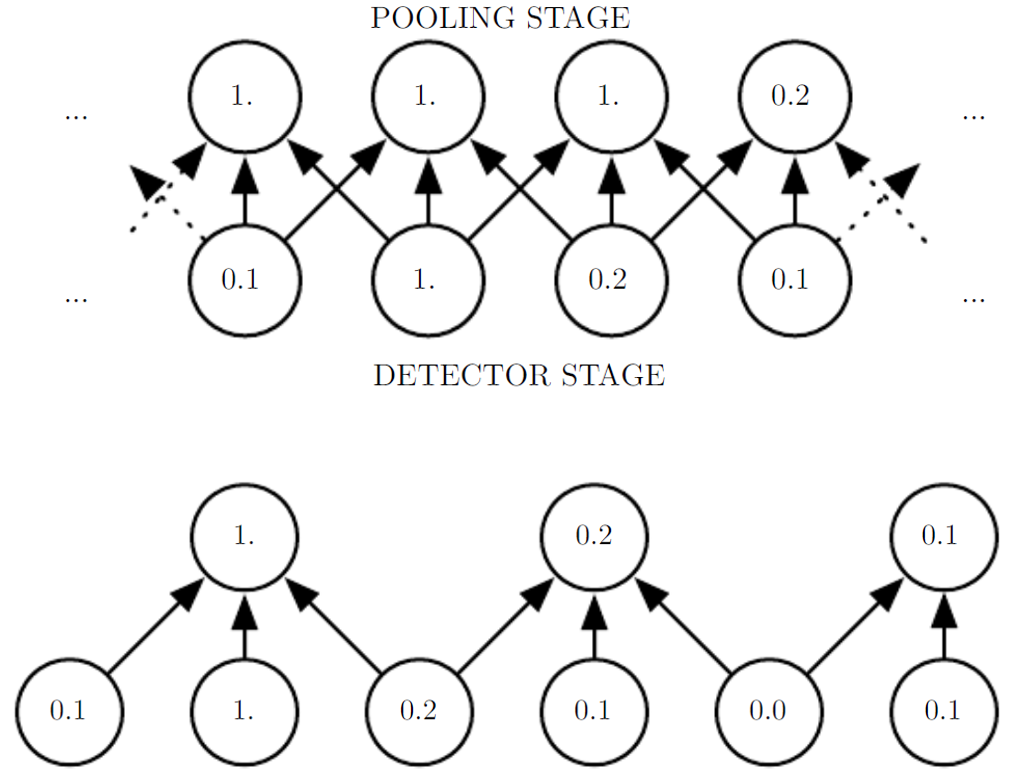
\includegraphics[width=0.8\linewidth]{images/stride.PNG}
	\end{figure}
	\begin{figure}[H]
		\centering
		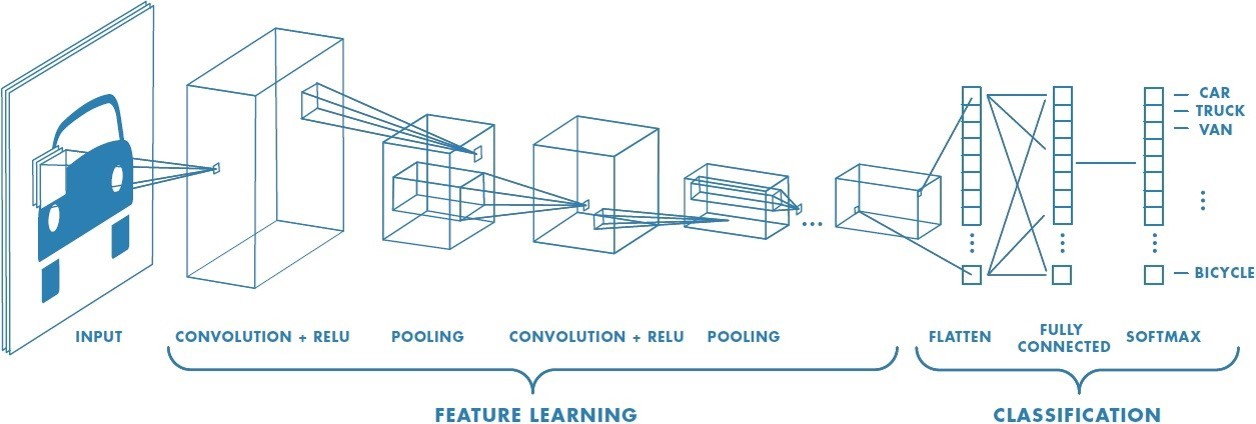
\includegraphics[width=0.9\linewidth]{images/cnn_arch.jpg}
	\end{figure}
	\newpage
	\subsection{Variants of the Basic Convolution Function}
	Assume we have a 4D kernel tensor $\tK$ with element $\etK_{i,j,k,l}$ giving the connection strength between a unit in channel $i$ of the output and a unit in channel $j$ of the input, with an offset of $k$ rows und $l$ columns between the output and input unit.\\
	Assume our input consists of observed data $\tV$ with element $\etV_{i,j,k}$ giving the value of the input unit within channel $i$ at row $j$ and column $k$.
	\[ \tZ_{i,j,k} = \sum_{l,m,n} \etV_{l,j+m-1,k+n-1} \etK_{i,l,m,n} \]

	Choosing a stride bigger than one results in reduction of computational cost.
	We can think of this as \textbf{downsampling} the output of the full convolution function.\\
	If we want to sample only every $s$ (stride) pixels in each direction in the output, then we can define a downsampled convolution function $c$ as
	\[ \etZ_{i,j,k} = c(\tK,\tV,s)_{i,j,k} = \sum_{l,m,n}\left[ \etV_{l,(j-1)\times s+m,(k-1)\times s+n} \etK_{i,l,m,n} \right] \]
	\begin{figure}[H]
		\centering
		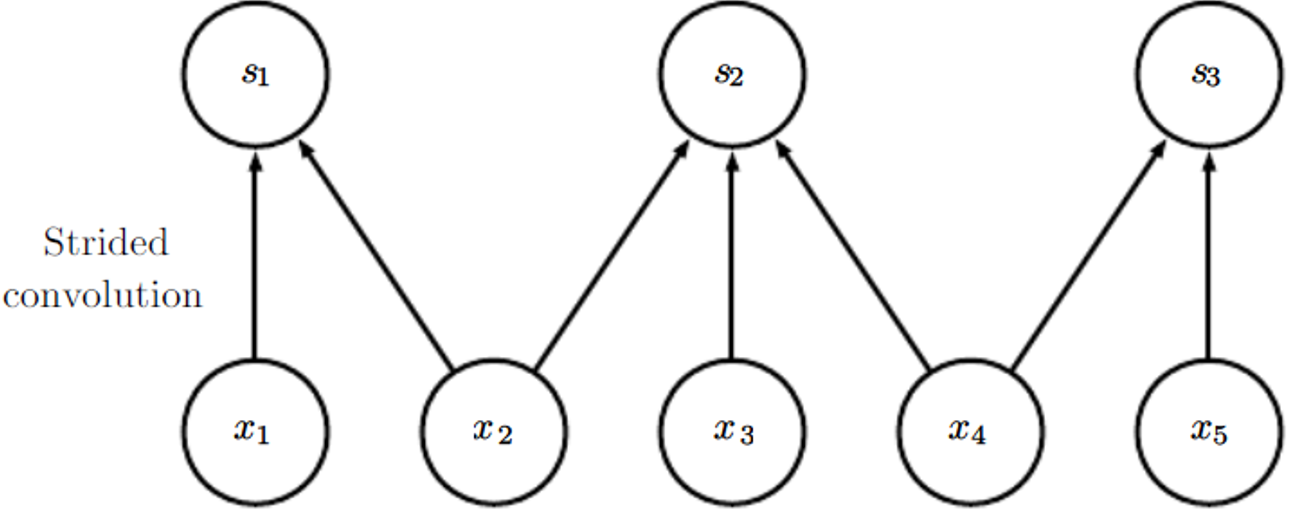
\includegraphics[width=0.5\linewidth]{images/strided_conv.PNG}
	\end{figure}

	One essential feature of any CNN implementation is the ability to\textbf{ implicitly zero-pad} the input $\tV$ in order to make it wider.
	Without this feature, the width of the representation shrinks by one pixel less than the kernel width at each layer:
	\[ \underbrace{(m\times n)}_{\text{Input}} \ast \underbrace{(k\times k)}_{\text{Kernel}} =
	\underbrace{\left( (m-k+1)\times (n-k+1) \right)}_{\text{Output}} \]
	Three special cases of zero-padding:
	\begin{enumerate}
		\item No zero-padding, therefore the convolution kernel is only allowed to visit positions where the entire kernel is contained \textbf{entirely} within the image. In MATLAB terminology, this is called \textbf{valid} convolution. In this case, all pixels in the output are a function of the same number of pixels in the input.
		\item Just enough zero-padding is added to keep the size of the output equal to the size of the input. MATLAB calls this \textbf{same} convolution. In this case, the network can contain as many convolutional layers as the available hardware can support. However, the input pixels near the border influence fewer output pixels than the input pixels further to the center. This can make the border pixels somewhat underrepresented in the model.
		\item The last one is called \textbf{full} convolution (in MATLAB), where enough zeroes are added for every pixel to be visited $k$ times in each direction, resulting in an output image of width $m+k-1$. In this case, the output pixels near the border are a function of fewer pixels than the output pixels near the center. This can make it difficult to learn a single kernel that performs well at all positions in the convolutional feature map.
		\item[$\rightarrow$] Usually, the optimal amount of zero padding (in terms of test set classification accuracy) lies somewhere \textbf{between valid and same} convolution.
	\end{enumerate}

	\textbf{Locally connected layers}  are not convolutional layers, even though they are locally connected but not with shared weights.
	In this case, the adjacency matrix in the MLP graph is the same, but every connection has its own weight, specified by a 6D tensor $\tW$.
	The indices into $\tW$ are respectively:
	$i$ the output channel, $j$ the output row, $k$ the output column, $l$ the input channel, $m$ the row offset within the input, $n$ the column offset within the input.
	The linear part of a locally connected layer is given by
	\[ \etZ_{i,j,k} = \sum_{l,m,n} \left[ \etV_{l,j+m-1,k+n-1} w_{i,j,k,l,m,n} \right] \]
	This is sometimes also called \textbf{unshared convolution}, because it is a similar operation to discrete convolution with a small kernel, but without sharing parameters across locations.
	Locally connected layers are useful when we know that each feature should be a function of a small part of space, but there is no reason to think that the same feature should occur across all of space.
	For example, if we want to tell if an image is a picture of a face, we only need to look for the mouth in the bottom half of the image.
	\begin{figure}[H]
		\centering
		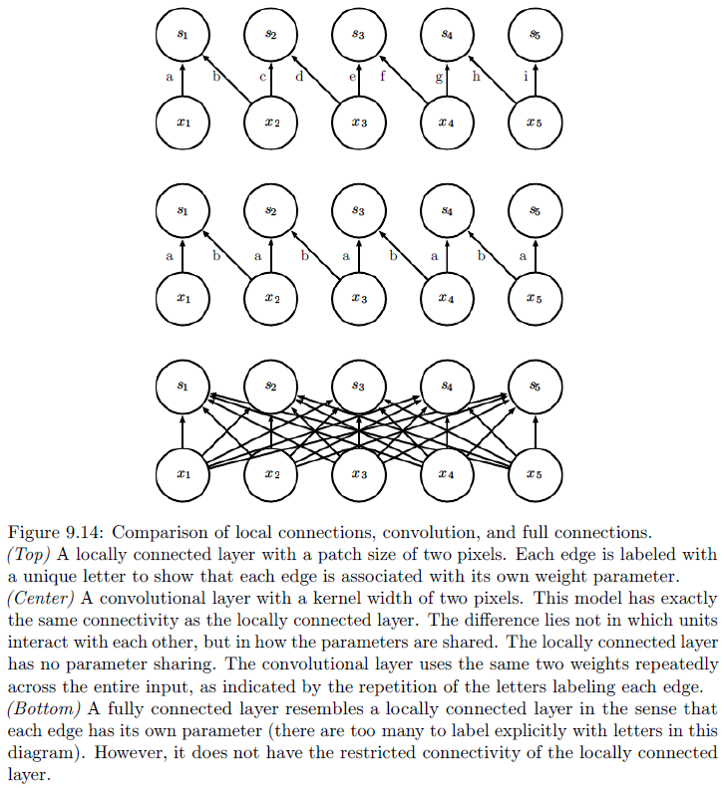
\includegraphics[width=0.8\linewidth]{images/locallyConn.png}
	\end{figure}
	\newpage
	\subsection{Data Types}
	The data used with a CNN usually consists of several channels, each channel being the observation of a different quantity at some point in space or time.
	\begin{figure}[H]
		\centering
		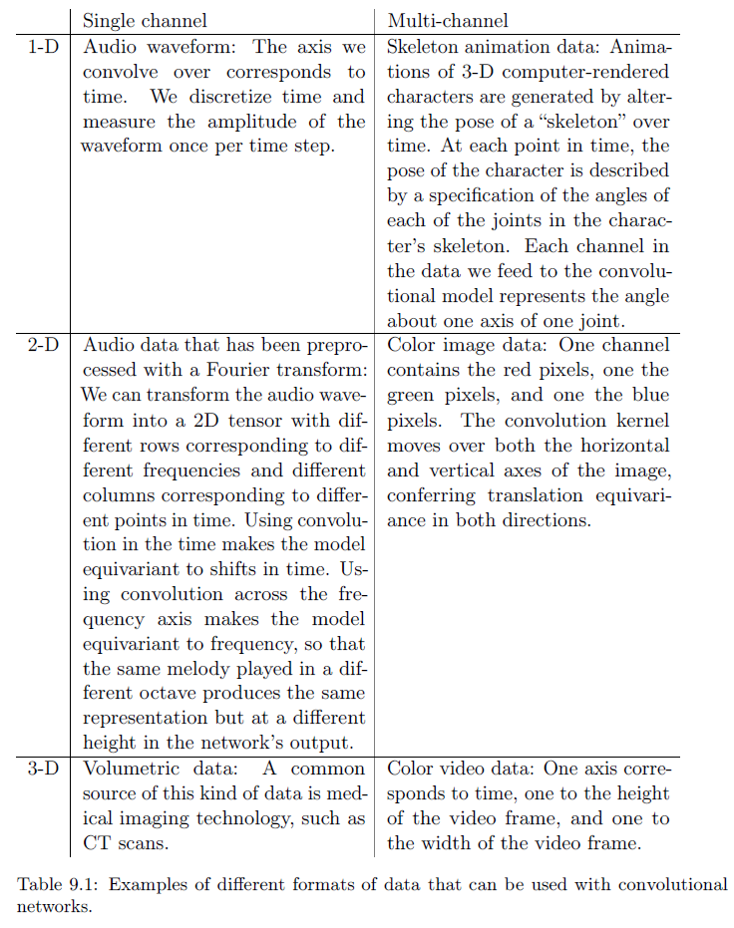
\includegraphics[width=\linewidth]{images/datatypes.png}
	\end{figure}

	One advantage to CNNs is that they can also process inputs with \textbf{varying spatial extents}.
	These kinds of input simply cannot be represented by traditional, matrix multiplication-based neural networks.
	Sometimes the output of the network is allowed to have variable size as well as the input, for example if we want to assign a class label to each pixel of the input.
	In other cases, the network must produce some fixed-size output, for example if we want to assign a single class label to the entire image. In this case, we must make some additional design steps, like inserting a pooling layer whose \textbf{pooling regions scale in size proportional to the size of the input}, in order to maintain a fixed number of pooled outputs.
	\columnbreak
	\subsection{Efficient Convolution Algorithms}
	Convolution is equivalent to converting both the input and the kernel to the frequency domain using a \textbf{Fourier transform (FFT)}, performing point-wise multiplication of the two signals, and converting back to the time domain using an inverse Fourier transform. For some problem sizes, this can be faster than the naive implementation of discrete convolution.\\

	When a d-dimensional kernel can be expressed as the outer product of d vectors, one vector per dimension, the kernel is called \textbf{separable}.
	Not only are two 1D convolutions much faster than one 2D convolution, the kernel also takes fewer parameters to represent as vectors.
	If the kernel is $w$ elements wide in each dimension, then naive multidimensional convolution requires $O(w^d)$ runtime and parameter storage space, while separable convolution requires $O(w\cdot d)$ runtime and parameter storage space.

	\begin{figure}[H]
		\centering
		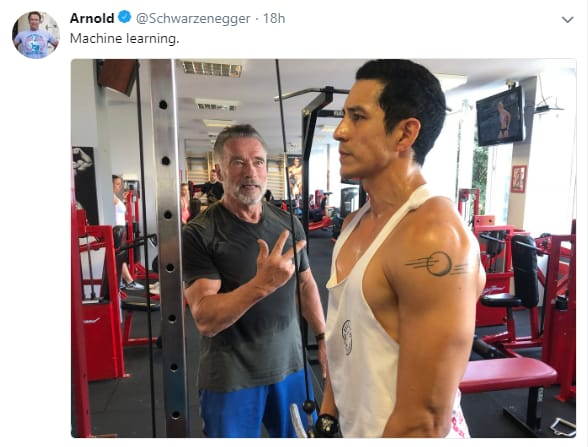
\includegraphics[width=0.9\linewidth]{images/arni.jpeg}
	\end{figure}

\end{multicols}

\newpage
